\documentclass[12pt,reqno,final,pdftex]{amsart}\usepackage[]{graphicx}\usepackage[]{color}
%% maxwidth is the original width if it is less than linewidth
%% otherwise use linewidth (to make sure the graphics do not exceed the margin)
\makeatletter
\def\maxwidth{ %
  \ifdim\Gin@nat@width>\linewidth
    \linewidth
  \else
    \Gin@nat@width
  \fi
}
\makeatother

\definecolor{fgcolor}{rgb}{0.345, 0.345, 0.345}
\newcommand{\hlnum}[1]{\textcolor[rgb]{0.686,0.059,0.569}{#1}}%
\newcommand{\hlstr}[1]{\textcolor[rgb]{0.192,0.494,0.8}{#1}}%
\newcommand{\hlcom}[1]{\textcolor[rgb]{0.678,0.584,0.686}{\textit{#1}}}%
\newcommand{\hlopt}[1]{\textcolor[rgb]{0,0,0}{#1}}%
\newcommand{\hlstd}[1]{\textcolor[rgb]{0.345,0.345,0.345}{#1}}%
\newcommand{\hlkwa}[1]{\textcolor[rgb]{0.161,0.373,0.58}{\textbf{#1}}}%
\newcommand{\hlkwb}[1]{\textcolor[rgb]{0.69,0.353,0.396}{#1}}%
\newcommand{\hlkwc}[1]{\textcolor[rgb]{0.333,0.667,0.333}{#1}}%
\newcommand{\hlkwd}[1]{\textcolor[rgb]{0.737,0.353,0.396}{\textbf{#1}}}%

\usepackage{framed}
\makeatletter
\newenvironment{kframe}{%
 \def\at@end@of@kframe{}%
 \ifinner\ifhmode%
  \def\at@end@of@kframe{\end{minipage}}%
  \begin{minipage}{\columnwidth}%
 \fi\fi%
 \def\FrameCommand##1{\hskip\@totalleftmargin \hskip-\fboxsep
 \colorbox{shadecolor}{##1}\hskip-\fboxsep
     % There is no \\@totalrightmargin, so:
     \hskip-\linewidth \hskip-\@totalleftmargin \hskip\columnwidth}%
 \MakeFramed {\advance\hsize-\width
   \@totalleftmargin\z@ \linewidth\hsize
   \@setminipage}}%
 {\par\unskip\endMakeFramed%
 \at@end@of@kframe}
\makeatother

\definecolor{shadecolor}{rgb}{.97, .97, .97}
\definecolor{messagecolor}{rgb}{0, 0, 0}
\definecolor{warningcolor}{rgb}{1, 0, 1}
\definecolor{errorcolor}{rgb}{1, 0, 0}
\newenvironment{knitrout}{}{} % an empty environment to be redefined in TeX

\usepackage{alltt}
%% DO NOT DELETE OR CHANGE THE FOLLOWING TWO LINES!
%% $Revision$
%% $Date$
\usepackage[round,sort,elide]{natbib}
\usepackage{graphicx}
\usepackage{times}
\usepackage{rotating}
\usepackage{subfig}
\usepackage{color}
\newcommand{\aak}[1]{\textcolor{cyan}{#1}}
\newcommand{\mab}[1]{\textcolor{red}{#1}}
\newcommand{\cec}[1]{\textcolor{blue}{#1}}

\setlength{\textwidth}{6.25in}
\setlength{\textheight}{8.75in}
\setlength{\evensidemargin}{0in}
\setlength{\oddsidemargin}{0in}
\setlength{\topmargin}{-.35in}
\setlength{\parskip}{.1in}
\setlength{\parindent}{0in}

%% cleveref must be last loaded package
\usepackage[sort&compress]{cleveref}
\crefname{figure}{Fig.}{Figs.}
\Crefname{figure}{Fig.}{Figs.}
\crefname{table}{Table}{Tables}
\Crefname{table}{Tab.}{Tables}
\crefname{equation}{Eq.}{Eqs.}
\Crefname{equation}{Eq.}{Eqs.}
\crefname{appendix}{Appendix}{Appendices}
\Crefname{appendix}{Appendix}{Appendices}
\creflabelformat{equation}{#2#1#3}
\newcommand{\crefrangeconjunction}{--}
\newcommand{\creflastconjunction}{, and~}

\theoremstyle{plain}
\newtheorem{thm}{Theorem}
\newtheorem{corol}[thm]{Corollary}
\newtheorem{prop}[thm]{Proposition}
\newtheorem{lemma}[thm]{Lemma}
\newtheorem{defn}[thm]{Definition}
\newtheorem{hyp}[thm]{Hypothesis}
\newtheorem{example}[thm]{Example}
\newtheorem{conj}[thm]{Conjecture}
\newtheorem{algorithm}[thm]{Algorithm}
\newtheorem{remark}{Remark}
\renewcommand\thethm{\arabic{thm}}
\renewcommand{\theremark}{}

\numberwithin{equation}{part}
\renewcommand\theequation{\arabic{equation}}
\renewcommand\thesection{\arabic{section}}
\renewcommand\thesubsection{\thesection.\arabic{subsection}}
\renewcommand\thefigure{\arabic{figure}}
\renewcommand\thetable{\arabic{table}}
\renewcommand\thefootnote{\arabic{footnote}}

\newcommand\scinot[2]{$#1 \times 10^{#2}$}
\newcommand{\code}[1]{\texttt{#1}}
\newcommand{\pkg}[1]{\textsf{#1}}
\newcommand{\dlta}[1]{{\Delta}{#1}}
\newcommand{\Prob}[1]{\mathbb{P}\left[#1\right]}
\newcommand{\Expect}[1]{\mathbb{E}\left[#1\right]}
\newcommand{\Var}[1]{\mathrm{Var}\left[#1\right]}
\newcommand{\dd}[1]{\mathrm{d}{#1}}
\newcommand{\citetpos}[1]{\citeauthor{#1}'s \citeyearpar{#1}}
\IfFileExists{upquote.sty}{\usepackage{upquote}}{}
\begin{document}



\begin{figure}
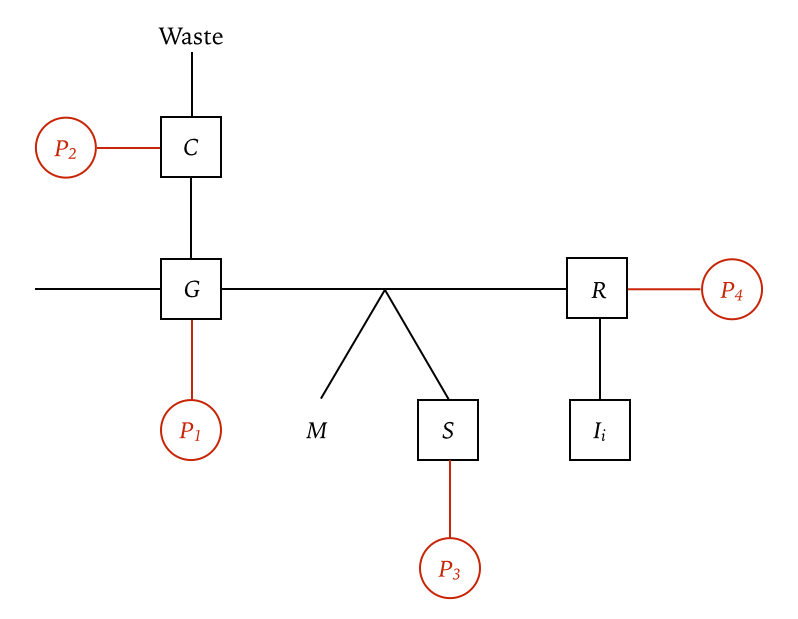
\includegraphics[width=\textwidth]{Macroparasite_DEB.png}
\caption{The basic model structure showing the state variables for the host (in boxes) and parasite (in circles). See the text for full details.}
\label{fig:model}
\end{figure}

The basic model (shown in Fig. \ref{fig:model}) defines five individual host state variables: $G(t)$, the biomass of ingested food in the ``gut''; $C(t)$, the biomass of unassimilated food in the ``colon''; $S(t)$, the structural biomass; $R(t)$, the reserve biomass; and $I_i(t)$, the biomass of the induced immune system.
We also need to consider the biomass of the constitutive immune system, $I_c(t)$, but as we discuss below, this has a very simple dependence on the other state variables.
There is also one state variable for the parasite biomass, $P(t)$, and we consider four possible ways that the parasite's can access host biomass.

A couple of notes.
$G(t)$ can be thought of as all of the ingested food that is still being processed by the host (it has neither been assimilated or lost as waste).
$C(t)$ is all of the unassimilated food - it is still in the gut (biologically), but is no longer available to the host.
$I_c(t)$ is the total biomass of all of the immune cells present in a host prior to parasite invasion, regardless of whether these cells are part of the innate immune system (e.g., eosinophils, macrophages) or the adaptive immune system (e.g., lymphocytes).
Similarly, $I_i(t)$ is the total biomass of all the immune cells produced in response to parasite invasion, regardless of their specific type.

The reason for including $G(t)$ and $C(t)$ is that it allows different parasites to have equivalent dynamical equations (as we will see below).
Previous versions of the model had the $P_1$ parasitizing the \emph{flow} of biomass through ingestion and $P_2$ parasitizing the \emph{flow} of biomass to waste, whereas $P_3$ and $P_4$ parasitize \emph{stored} biomass.
Thus, the parameters of different parasite growth equations had different units and were not totally comparable (at least in my head).
By considering biomass stored in the ``gut'' and ``colon,'' however, all of the parasites have equivalent parameters.

We make the assumption that we are modeling the biology of animals with determinant growth, so we move away from the standard DEB model assumptions.
In particular, we make some very strong assumptions about the growth of structural biomass and constitutive immune biomass.

\subsection*{Model assumptions:}
\begin{itemize}
\item individuals have a genetically predetermined growth pattern in structural biomass that is independent of how much they are eating;
\item individuals have a genetically predetermined constitutive immune system that depends only on the total weight $(S(t)+R(t))$ of the organism, not on how much they are eating;
\item total maintenance costs depend on the total weight and the biomasses of the constitutive and induced immune systems;
\item all assimilated biomass that is not used for maintenance or structural growth is stored in reserves;
\item the induced immune response ``paid'' using reserve biomass.
\end{itemize}

\subsection*{Ingestion}
We can consider a couple of different models of ingestion.
Since we are considering \emph{ad lib} feeding right now, we can ignore the fact that ingestion rate should be nonlinearly related to food abundance (e.g., by a Type II functional response), as food abundance is always saturating.
Then the simplest model would assume that ingestion is completely independent of anything related to individual state.
\citet{vanLeeuwen2002}, looking at data from mice, suggest that mice raised under \emph{ad lib} feeding conditions have an ingestion rate that is independent of age, size, or condition.
That would suggest that a reasonable model of ingestion rate $\iota$ is simply:
\begin{equation}
\iota = \iota_{\max},
\end{equation}
where $\iota_{\max}$ is the maximum ingestion rate.

On the other, standard DEB assumptions are that ingestion should scale with the surface area of structure, that is, with $S(t)^{2/3}$.
In this case, ingestion rate is
\begin{equation}
\iota=\iota_{\max }S^{2/3},
\end{equation}
where $\iota_{\max}$ is now the \emph{surface-area-specific} maximum ingestion rate (so it does not have the same units as $\iota_{\max}$ in the previous model.

However, \citet{deRoos2013} suggest that for demand-driven systems (where ingestion is adjusted to meet the individual's demands for resources), ingestion rate should depend on both size and body condition, as measured by the ratio of structure to reserves.
For animals feeding on super-abundant food, their model for ingestion rate is
\begin{equation}
\iota = \frac{2M_c/H_c}{1 + \exp\left(\eta(R/S-\theta)\right)}S^{2/3},
\end{equation}
where $\theta$ is the ``target'' body condition (ratio of reserve to structure); $\eta$ is a parameter that determines how quickly ingestion rate accelerates when $R/S$ drops below $\theta$; $M_c$ is the scaling constant of maximum ingestion rate with $S^{2/3}$; and $H_c$ is the half-saturation resource density.
For simplicity, we will combine $2M_c/H_c$ into a single parameter $\iota_{\max}$, so the model is then
\begin{equation}
\iota = \frac{\iota_{\max}S^{2/3}}{1 + \exp\left(\eta(R/S-\theta)\right)}.
\end{equation}


\subsection*{Dynamics of food biomass in the gut}
Ingested food biomass is temporarily stored in the gut, where it is processed.
Biomass that leaves the gut is either assimilated or excreted as waste (stopping temporarily in $C(t)$).
Thus,
\begin{equation}
\frac{dG}{dt} = \iota - \rho G,
\end{equation}
where $\rho$ is the rate food biomass leaves the gut ($1/\rho$ is therefore the mean gut transit time).
We assume that a fraction of this biomass is assimilated, and the remainder move onto $C$.

\subsection*{Dynamics of food biomass in the ``colon''}
Let $\rho (1-\epsilon_A) G$ be the rate that undigested food enters the ``colon''.
In reality, there is likely some relationship between $\epsilon_A$ and $\rho$: assimilation efficiency should increase as gut transit time slows down.
Moreover, many parasites will influence $\epsilon_A$; in fact, if an organism doesn't reduce $\epsilon_A$, it isn't really a parasite at all.
Since we have defined $\rho$ to be the gut transit time, and in reality we are still in the gut, undigested biomass should leave this compartment at the same rate as it enters.
This makes the model,
\begin{equation}
\frac{dC}{dt} = \rho (1-\epsilon_A)G - \rho C.
\end{equation}

\subsection*{Reserve dynamics}
The key equation for host dynamics is the equation for reserve dynamics, which is
\begin{equation}
\frac{dR}{dt}=\epsilon _R\left(\rho \epsilon_A G-M-C_G\right)-b R P,
\end{equation}
where $M$ is the total maintenance rate, $C_G$ is the cost of growth in structural biomass, $\epsilon _R$ is the cost of converting assimilated biomass into reserve biomass, and $bRP$ is the allocation of reserve to fuel an induced immune response.
Note that this last assumption makes the induced response independent of the number of induced (or constitutive) immune cells.
This kind of model has been studied by other authors \citep{Bonhoeffer1994,Alizon2005,Fenton2006,Hamilton2008}, and reflects the fact that the immune-parasite interaction is not really a predator-prey interaction in the sense that the immune response is not stimulated by direction contact between immune cells and parasites.

\subsection*{Maintenance}
An organism must pay the metabolic cost of all of its cells, which means that a reasonable model of maintenance is
\begin{equation}
M=m(S+R)+m_cI_c+m_iI_i,
\end{equation}
where $m$ is the maintenance rate for weight, which is assumed to be the same for structure and reserves, $m_c$ is the maintenance rate for constitutive immune biomass, and $m_i$ is the maintenance rate for induced immune biomass.
On the one hand, it seems like $m_c=m_i$ because the cells that are produced during the induced immune response are simply clones of those cells of the constitutive immune population that reacted to the antigen.
However, that is not the case because the production of constitutive immune cells is very wasteful: for every 100 immune cells produced by the thymus, 95 are destroyed immediately, either because they won't work with MHC or because they are self-reactive.
Thus, the cost of maintaining an effective constitutive immune cell should be much higher than the cost of maintaining an effective induced immune cell, even though biologically, they are clones.
Assuming the 95\% figure is reliable, it is reasonable to imagine that the maintenance cost for 1g of constitutive immune biomass is 20-fold higher than the cost of maintaining 1g of induced immune biomass.

It may be worth questioning whether there should be separate maintenance rates for structure $S(t)$ versus reserves $R(t)$, but this is probably reasonable for the moment.
I discuss the separate maintenance costs for constitutive versus induced immune biomass below.

\subsection*{Constitutive immune defense}
Rather than considering a dynamic constitutive immune defense, we instead assume that organisms maintain a constitutive immune biomass that is proportional to total biomass.
To some extent, this makes biological sense: hosts should want to maintain a relatively constant level of surveillance, regardless of how much tissue they have.
At least some theoretical evidence supports this assumption \citep{Wiegel2004}.
Therefore, we assume that the total biomass of constitutive defense is:
\begin{equation}
I_c=k(S+R),
\end{equation}
where $k$ is the biomass of the constitutive immune system relative to the total biomass in weight ($k<<1$).

Note that we do not consider the cost of building these cells, or, more precisely, we assume that the building cost and the maintenance cost are identical.
This is reasonably well-supported by data, according to Andrea: as noted above, these cells are constantly being produced by a very wasteful process; moreover, these cells have a fairly short half-life, resulting in very fast turnover of the entire population.
All of this dynamic can be captured reasonably well by simply assuming that the standing army of effective constitutive immune cells is tied to total mass of the host.
This is quite different from our assumptions for the induced immune response (discussed below).

\subsection*{ Induced immune response}
The derivation of the reserve dynamics equation implies a model for the induced immune response of
\begin{equation}
\frac{dI_i}{dt}=\epsilon _ib R P-\mu _II_i,
\end{equation}
where $\epsilon _i$ is the cost of converting reserve biomass into \textit{effective} induced immune biomass (see below), $b$ is the rate reserve biomass is allocated to the immune system per unit of parasite biomass, and $\mu _I$ is the background rate that immune cells are lost.

With this model formulation, if an infection is cleared, the induced immune response returns to 0; we may, at some point in the future, want to consider the fact that some of the cells of the induced immune response become part of the constitutive immune system after infection (e.g., memory cells).

We can also make some assumptions about parameter values and model initial conditions.
According to Perelson, the probability that a lymphocyte (for example) of the constitutive immune system will react with any particular epitope is very small, on the order of $10^{-5}$.
This suggests that the initial condition of the induced immune system is $10^{-5}I_c$.
The rate of proliferation will depend on $\epsilon_i b$, which may be possible to find estimates for in the published literature; finding the estimate of $b$ or $\epsilon_i$ by itself might be more challenging.

Andrea has suggested the work of Rob de Boer and Andrew Yates for models of immune cell proliferation (and killing too).
There is also some nice stuff by Kirk Klasing looking at the energetic/protein cost of the innate and induced immune response.

\subsection*{Cost of growth}
This one turns out be slightly more complicated.
Let's start with the equation for structural biomass.

If you assume that structural biomass $S$ scales with structural length $L$ as $S =\epsilon L^3$, and you assume that structural length
follows a von Bertalanffy equation, then
\begin{align}
\frac{dS}{dt} &=\frac{d\left(\alpha L^3\right)}{\text{dt}} \\
& =3\alpha  L^2 \frac{dL}{dt} \\
& =3 \alpha  L^2 \left(\gamma \left(L_{\infty}-L\right)\right) \\
& =3 \gamma \left(\alpha  L^2 L_{\infty}-\epsilon  L^3\right) \\
& =3 \gamma \left(\alpha  L^2L_{\infty }-S\right).
\end{align}

Note that $S^{2/3}=\alpha^{2/3}L^2$, or $L^2=S^{2/3}/\alpha^{2/3}$, so
\begin{equation}
\frac{dS}{dt}=3\gamma  \left(\alpha^{1/3}L_{\infty }S^{2/3}-S\right).
\end{equation}
If a unit of structural biomass increase costs $\epsilon_G$, then the total cost for structural growth is
\begin{equation}
C_G = \epsilon _G 3\gamma  \left(\alpha ^{1/3}L_{\infty }S^{2/3}-S\right).
\end{equation}
This agrees with Anieke's derivation.
Most of these parameters have probably already been estimated (for mice, anyway; see the back of Kooijman's book), including the shape parameter $\alpha$, the maximum structural length $L_{\infty }$, and the growth rate in structure $\gamma$.

Of course, it is possible to directly solve the von Bertalanffy growth equation, so we could eliminate one equation from the model by simply solving for the size of the animal at any age.
In particular, $\frac{dL}{dt}=\gamma \left(L_{\infty }-L\right), \text{with} L(0)=L_b$, has the solution $L(t)=L_{\infty }+\left(L_b-L_{\infty}\right)e^{-\gamma t}$, and the structural biomass $S(t)=\alpha L(t)^3$.

However, if the parasite utilizes structure as a resource, the structural growth equation has to be modified to include parasitism, and we will no longer be able to solve the equation.
In particular, the structural biomass equation will become
\begin{equation}
\frac{dS}{dt}=3\gamma  \left(\alpha^{1/3}L_{\infty }S^{2/3}-S\right)-\frac{\sigma_S S P_3}{H_S+S}.
\end{equation}
However, we can still make use of the analytical solution: when the parasite is using up structural biomass as resource, the amount allocated to growth (i.e., $C_G$)should increase in proportion to how far the host is from it's target structural biomass.
That is, define
\begin{equation}
S_{\text{target}}(t)=\alpha \left(\left(L_b-L_{\infty }\right) e^{-\gamma  t}+L_{\infty }\right)^3,
\end{equation} and let the solution of the differential equation for $\frac{dS}{dt}$ give the actual weight.

It makes sense to me, at this point, to imagine that what happens when an organism is below its target structural biomass is that it increases the amount of energy allocated to growth to accelerate its growth rate (e.g., engage in ``catch-up'' growth).
Mathematically, that could be accomplished by making the parameter $\gamma$ a function of the difference between the target structural biomass and the actual structural biomass.
For example, if you let
\begin{equation}
\gamma =\gamma _{\min }+\gamma _{\text{catchup}}\left(\frac{S_{\text{target}}(t)}{S(t)}-1\right),
\end{equation}
then whenever $S(t)<S_{\text{target}}(t)$, $\gamma$ increases, increasing the allocation of energy towards growth and enabling the \textit{possibility} of catch-up growth.
Of course, if there is a parasite that is also sucking up biomass, the host may or may not actually be able to catch up.
If the parasite is cleared, the host will have an increased growth rate until $S(t)=S_{\text{target}}(t)$, and then the growth rate will fall back to normal.

Thus, we have equations for the rate of structural biomass increase, the growth rate, and cost of growth:
\begin{align}
\frac{dS}{dt} &= 3\gamma  \left(\alpha^{1/3}L_{\infty }S(t)^{2/3}-S(t)\right)-\frac{k S(t) P(t)}{h+S(t)} \\
C_G(t)&=\epsilon_G 3\gamma \left(\alpha^{1/3}L_{\infty }S(t)^{2/3}-S(t)\right) \\
\gamma(S) &=\gamma_{\min}+\gamma_{\text{catchup}}\left(\frac{S_{\text{target}}(t)}{S(t)}-1\right) \\
S_{\text{target}}(t) &=\alpha \left(\left(L_b-L_{\infty }\right) e^{-\gamma  t}+L_{\infty }\right)^3
\end{align}
For non-parasitized hosts, or hosts parasitized by parasites targeting other sources of biomass, then $S(t)=S_{\text{target}}(t)$, and you only need two of the above equations.

\subsection*{Host mortality}
The last consideration is of host mortality rate.
DEB theory has been used extensively to consider how metabolic activity relates to mortality risk \citep[by keeping track of things like oxidative damage, e.g.,][]{vanLeeuwen2002,Kooijman2009}, but that might be more complicated than we wish to deal with at the moment.
A simpler solution is to imagine that, given its structural volume, an organism has a ``target'' amount of reserves that it seeks to maintain.
This is known, in the dynamic energy budget literature, as the ``weak homeostasis assumption.''
It can be modelled as:
\begin{equation}
\frac{d\mu}{dt} = \mu_{\min} + \mu_{accel}\max\left(\theta \frac{S}{R}-1, 0\right),
\end{equation}
where $\mu_{\min}$ is the baseline mortality rate of a healthy host (which we assume for simplicity is independent of age), $\mu_{accel}$ is the rate that mortality accelerates with decreasing body condition, and $\theta$ is the target ratio of reserves $R$ to structure $S$ (as above in the resource ingestion rate equation).
With this formulation, as $R$ approaches zero, mortality rate accelerates dramatically.
The parameter $\theta$ allows mortality rate to accelerate well before $R$ actually gets close to zero, which is likely quite biologically reasonable.
A slightly simplified version of this would be
\begin{equation}
\frac{d\mu}{dt} = \mu_{\min} + \mu_{R}\left(\theta \frac{S}{R} - 1\right),
\end{equation}
which allows mortality rate to \emph{fall} when $R$ is large relative to $S$.
This may not be particularly biologically reasonable, given the negative health consequences of obesity, but does make the system a bit more analytically tractable.

\section*{Model equations, including parasitism}
As seen in Fig. \ref{fig:model}, we consider 4 kinds of parasite: $P_1$ are parasites of ingestion; $P_2$ are parasites of waste; $P_3$ are parasites of structure; and $P_4$ are parasites of reserves.
By allowing the existence of a gut and colon, all four of these parasites can bemodelled with an equivalent mathematical formulation:
\begin{equation}
\frac{dP_j}{dt} = \epsilon_P \frac{\sigma P_j E_j}{H_j+E_j}  - \mu_P P_j - \mu_c P_j I_c - \mu_i P_j I_i,
\end{equation}
where $j$ refers the parasite class and $E_j$ is the parasite's source of energy: either $G(t)$ (for $j=1$), $C(t)$ (for $j=2$), $S(t)$ (for $j=3$), or $R(t)$ (for $j=4$).
The parameters are: $\epsilon_P$ is the cost of converting a gram of stolen host biomass into a gram of parasite biomass, which likely varies with parasite type; $\sigma$ is the parasite's rate of biomass consumption; $\mu_P$ is the parasite's background rate of biomass loss; $\mu_c$ and $\mu_i$ are the biomass loss rates due to interaction with the constitutive and induced immune responses, respectively.

The full model (assuming the demand-driven ingestion rate function):
\begin{align}
\frac{dG}{dt} &= \frac{\iota_{\max}S^{2/3}}{1 + \exp\left(\eta(R/S-\theta)\right)} - \rho G - \frac{\sigma_G P_1 G}{H_G + G}, \\
\frac{dC}{dt} &= \rho (1-\epsilon_A)G - \rho C - \frac{\sigma_C P_2 C}{H_C + C}, \\
\frac{dS}{dt} &= 3\gamma(S) \left(\alpha^{1/3}L_{\infty }S^{2/3}-S\right) - \frac{\sigma_S P_3 S}{H_S + S}, \\
\frac{dR}{dt} &= \epsilon_R\left(\rho \epsilon_A G-M(S,R,I_i)-C_G(S)\right)-b R (P_1+P_2+P_3+P_4) - \frac{\sigma_R P_4 R}{H_R + R}, \\
\frac{dI_i}{dt} &= \epsilon_ib R P-\mu_II_i, \\
\frac{d\mu}{dt} &= \mu_{\min} + \mu_{accel}\max\left(\theta \frac{S}{R} - 1, 0\right), \\
\frac{dP_1}{dt} &= \epsilon_P \frac{\sigma_G P_1 G}{H_G + G} - \mu_P P_1 - \mu_c I_c P_1 - \mu_i I_i P_1, \\
\frac{dP_2}{dt} &= \epsilon_P \frac{\sigma_C P_2 C}{H_C + C} - \mu_P P_2 - \mu_c I_c P_2 - \mu_i I_i P_2, \\
\frac{dP_3}{dt} &= \epsilon_P \frac{\sigma_S P_3 S}{H_S + S} - \mu_P P_3 - \mu_c I_c P_3 - \mu_i I_i P_3, \\
\frac{dP_4}{dt} &= \epsilon_P \frac{\sigma_R P_4 R}{H_R + R} - \mu_P P_4 - \mu_c I_c P_4 - \mu_i I_i P_4.
\end{align}

The functions for maintenance rate, constitutive immune response, cost of growth, and structural growth rate are:
\begin{align}
M &= m(S+R)+m_cI_c+m_iI_i, \\
I_c &= k(S + R), \\
C_G(t)&=\epsilon_G 3\gamma(R) \left(\alpha^{1/3}L_{\infty }S(t)^{2/3}-S(t)\right), \\
\gamma(S) &=\gamma _{\min}+\gamma_{\text{catchup}}\left(\frac{S_{\text{target}}(t)}{S(t)}-1\right), \\
S_{\text{target}}(t) &= \alpha \left(\left(L_b-L_{\infty }\right) e^{-\gamma  t}+L_{\infty }\right)^3.
\end{align}




\section*{Interesting mathematical experiments}
\begin{itemize}
\item How much does a $P_2$ parasite have to reduce digestion efficiency before it becomes worthwhile to attack it rather than ignore it? Mounting an immune response to a parasite engenders a cost to the host by reducing $R$ (which accelerates mortality rate). Is it worthwhile to attack \emph{any} parasite that invades, or is it better to ignore some? This amounts to an argument about tolerance.
\end{itemize}

To model this, we need to consider how parasite biomass affects assimilation efficiency.
It is clear that we cannot simply assume that the presence of a parasite causes a \emph{fixed} decrease in assimilation efficiency, as there would be no point in fighting such a parasite because unless the parasite can be cleared, no advantage is gained by wasting energy fighting it.
It makes the most sense to imagine that parasite abundance has a saturating effect on digestion efficiency:
\begin{equation}
\epsilon_A(P_2) = \epsilon_A\left(1 - \frac{\epsilon_{A_{\min}} P_2}{H_\epsilon + P_2}\right).
\end{equation}
In the absence of parasites, assimilation efficiency is $\epsilon_A$, as above.
As parasite biomass increases, digestive efficiency falls; $\epsilon_{A_{\min}}$ gives the maximum possible reduction in digestive efficiency (bounded between 0 and 1, and more likely some value less than one).

Initially, for simplicity, I wanted to assume that ingestion depends linearly on structural biomass, to avoid the complexity of condition dependent ingestion, and in accordance with Sarah's data.
However, this does not work mathematically, and it is fairly straightforward to see why.
You can show that the equilibrium reserve biomass in the absence of parasitism, $R^*$, under such a model, is:
\begin{equation}
R^* = \left(\frac{\epsilon_A \iota_{\max}}{m + k m_c} - 1 \right) S^*.
\end{equation}
You can see why in the Mathematica notebook ``Macroparasite\_DEB\_analytics.nb.''
The ratio of reserves to structure is therefore equal to the term in parentheses.
On the basis of Sarah's data (and the simple general model in \citep{deRoos2013}), this ratio should be approximately 0.25.
That will happen when $\epsilon_A \iota_{\max} = 1.25(m + k m_c)$. Given that $\epsilon_A$ is a fraction close to unity in magnitude, this suggests that ingestion rate and maintenance rate should be quite close in value.
But this is ridiculous: maintenance rates should be on the order of ten-fold smaller than ingestion rates.
Thus, in a constant food environment with a determinantly growing organism, it is necessary to implement condition-dependent feeding.

Therefore, the model is:
\begin{align}
\frac{dG}{dt} &= \frac{\iota_{\max}S^{2/3}}{1 + \exp\left(\eta(R/S-\theta)\right)} - \rho G, \\
\frac{dC}{dt} &= \rho (1-\epsilon_A(P_2))G - \rho C - \frac{\sigma_C P_2 C}{H_C + C}, \\
\frac{dS}{dt} &= 3\gamma_{\min} \left(\alpha^{1/3}L_{\infty }S^{2/3}-S\right), \\
\frac{dR}{dt} &= \epsilon_R\left(\rho \epsilon_A(P_2) G-M(S,R,I_i)-C_G(S)\right)-b R P_2, \\
\frac{dI_i}{dt} &= \epsilon_ib R P-\mu_II_i, \\
\frac{d\mu}{dt} &= \mu_{\min} + \mu_{accel}\max\left(\theta \frac{S}{R} - 1, 0\right), \\
\frac{dP_2}{dt} &= \epsilon_P \frac{\sigma_C P_2 C}{H_C + C} - \mu_P P_2 - \mu_c I_c P_2 - \mu_i I_i P_2,
\end{align}
where
\begin{align}
M &= m(S+R)+m_cI_c+m_iI_i, \\
I_c &= k(S + R), \\
C_G(t)&=\epsilon_G 3 \gamma_{min}\left(\alpha^{1/3}L_{\infty }S(t)^{2/3}-S(t)\right), \\
\epsilon_A(P_2) &= \epsilon_A\left(1 - \frac{\epsilon_{A_{\min}} P_2}{H_\epsilon + P_2}\right).
\end{align}

\begin{knitrout}\scriptsize
\definecolor{shadecolor}{rgb}{0.969, 0.969, 0.969}\color{fgcolor}\begin{kframe}
\begin{alltt}
\hlkwd{require}\hlstd{(deSolve)}
\hlcom{## initial conditions: assuming 3.93g lean mass for every g of fat}
\hlcom{## mass, and a birth rate of 1.5 g}
\hlstd{y0} \hlkwb{<-} \hlkwd{c}\hlstd{(}\hlkwc{G}\hlstd{=}\hlnum{0}\hlstd{,} \hlkwc{C}\hlstd{=}\hlnum{0}\hlstd{,} \hlkwc{S}\hlstd{=}\hlnum{1.5}\hlopt{*}\hlnum{3.93}\hlopt{/}\hlnum{4.93}\hlstd{,} \hlkwc{R}\hlstd{=}\hlnum{1.5}\hlopt{*}\hlnum{1.93}\hlopt{/}\hlnum{4.93}\hlstd{,} \hlkwc{Ii}\hlstd{=}\hlnum{0}\hlstd{,} \hlkwc{mu}\hlstd{=}\hlnum{0}\hlstd{,} \hlkwc{P2}\hlstd{=}\hlnum{1e-6}\hlstd{)}

\hlcom{## Run for 664 days (when mortality occurs for healthy mouse)}
\hlstd{times} \hlkwb{<-} \hlkwd{seq}\hlstd{(}\hlnum{0}\hlstd{,} \hlnum{664}\hlstd{,} \hlnum{0.1}\hlstd{)}

\hlstd{plotall} \hlkwb{<-} \hlkwa{function}\hlstd{(}\hlkwc{x}\hlstd{) \{}
    \hlkwd{par}\hlstd{(}\hlkwc{mfrow}\hlstd{=}\hlkwd{c}\hlstd{(}\hlnum{3}\hlstd{,}\hlnum{3}\hlstd{),} \hlkwc{mar}\hlstd{=}\hlkwd{c}\hlstd{(}\hlnum{2}\hlstd{,}\hlnum{4}\hlstd{,}\hlnum{0.5}\hlstd{,}\hlnum{0.5}\hlstd{),} \hlkwc{oma}\hlstd{=}\hlkwd{rep}\hlstd{(}\hlnum{0.5}\hlstd{,}\hlnum{4}\hlstd{))}
    \hlstd{labels} \hlkwb{<-} \hlkwd{c}\hlstd{(}\hlstr{"Age"}\hlstd{,} \hlstr{"Gut biomass"}\hlstd{,} \hlstr{"Waste biomass"}\hlstd{,} \hlstr{"Structure biomass"}\hlstd{,}
                \hlstr{"Reserve biomass"}\hlstd{,} \hlstr{"Immune biomass"}\hlstd{,} \hlstr{"Cumulative hazard"}\hlstd{,}
                \hlstr{"Parasite biomass"}\hlstd{,} \hlstr{"Ingestion rate"}\hlstd{,} \hlstr{"Assimilation rate"}\hlstd{)}
    \hlkwa{for} \hlstd{(i} \hlkwa{in} \hlnum{2}\hlopt{:}\hlkwd{ncol}\hlstd{(x))}
        \hlkwd{plot}\hlstd{(x[,}\hlnum{1}\hlstd{], x[,i],} \hlkwc{xlab}\hlstd{=}\hlstr{''}\hlstd{,} \hlkwc{ylab}\hlstd{=labels[i],} \hlkwc{type}\hlstd{=}\hlstr{'l'}\hlstd{)}
\hlstd{\}}

\hlkwd{source}\hlstd{(}\hlstr{"Macroparasite_DEB_models.R"}\hlstd{)}
\hlcom{## See mathematica notebook to see the justification for these}
\hlcom{## parasite and constitutive defense parameters.}
\hlstd{pars} \hlkwb{<-} \hlkwd{c}\hlstd{(}\hlkwc{imax}\hlstd{=}\hlnum{2}\hlstd{,} \hlcom{## estimated on the basis of Sarah's data}
          \hlkwc{theta}\hlstd{=}\hlnum{1}\hlopt{/}\hlnum{3.93}\hlstd{,} \hlcom{## estimated on the basis of Sarah's data}
          \hlkwc{rho}\hlstd{=}\hlnum{2}\hlstd{,} \hlcom{## estimated on the basis of Sarah's data}
          \hlkwc{eta}\hlstd{=}\hlnum{10}\hlstd{,} \hlcom{## guestimate based on parasite-free body condition}
          \hlkwc{epsA}\hlstd{=}\hlnum{0.85}\hlstd{,} \hlcom{## estimate from data}
          \hlkwc{epsG}\hlstd{=}\hlnum{1}\hlstd{,} \hlcom{## total guess}
          \hlkwc{epsR}\hlstd{=}\hlnum{1}\hlstd{,} \hlcom{## total guess}
          \hlkwc{Linf}\hlstd{=}\hlnum{2.94}\hlstd{,} \hlcom{## from Kooijman}
          \hlkwc{alpha}\hlstd{=}\hlnum{1}\hlstd{,} \hlcom{## from Kooijman}
          \hlkwc{gmin}\hlstd{=}\hlnum{.02}\hlstd{,} \hlcom{## guestimate based on parasite-free body condition}
          \hlkwc{m}\hlstd{=}\hlnum{0.2}\hlstd{,} \hlcom{## guestimate based on imax}
          \hlkwc{mc}\hlstd{=}\hlnum{0.03}\hlstd{,} \hlcom{## made up}
          \hlkwc{mi}\hlstd{=}\hlnum{0.005}\hlstd{,} \hlcom{## guestimate based on imax}
          \hlkwc{k}\hlstd{=}\hlnum{4.9e-5}\hlstd{,} \hlcom{## estimated on the basis of Sarah's data}
          \hlkwc{b}\hlstd{=}\hlnum{5e-3}\hlstd{,} \hlcom{# probably should be pretty small, as reserve}
                  \hlcom{# biomass should not be greatly depleted by the}
                  \hlcom{# induced immune response}
          \hlkwc{ui}\hlstd{=}\hlnum{1}\hlopt{/}\hlnum{20}\hlstd{,} \hlcom{## based on avg lifespan of 20 days (for non-B-cell lymphocytes)}
          \hlkwc{umin}\hlstd{=}\hlnum{1}\hlopt{/}\hlnum{664}\hlstd{,} \hlcom{## based on avg host lifespan}
          \hlkwc{uacc}\hlstd{=}\hlnum{1}\hlopt{/}\hlnum{664}\hlstd{,} \hlcom{## made up}
          \hlkwc{epsP}\hlstd{=}\hlnum{0.15}\hlstd{,} \hlcom{## based on model analysis}
          \hlkwc{epsI}\hlstd{=}\hlnum{0.8}\hlstd{,} \hlcom{## total guess}
          \hlkwc{sigmaC}\hlstd{=}\hlnum{10}\hlstd{,} \hlcom{## based on model analysis}
          \hlkwc{hC}\hlstd{=}\hlnum{0.1}\hlstd{,} \hlcom{## based on model analysis}
          \hlkwc{uP}\hlstd{=}\hlnum{1}\hlstd{,} \hlcom{## based on model analysis}
          \hlkwc{uC}\hlstd{=}\hlnum{100}\hlstd{,} \hlcom{## guess}
          \hlkwc{uI}\hlstd{=}\hlnum{200}\hlstd{,} \hlcom{## total guess}
          \hlkwc{epsAmin}\hlstd{=}\hlnum{0.5}\hlstd{,} \hlcom{## total guess}
          \hlkwc{heps}\hlstd{=}\hlnum{1e-3}\hlstd{,} \hlcom{## total guess}
          \hlkwc{tInf}\hlstd{=}\hlnum{Inf}\hlstd{)} \hlcom{## no infection}
\hlstd{out1} \hlkwb{<-} \hlkwd{ode}\hlstd{(}\hlkwc{y}\hlstd{=y0,} \hlkwc{times}\hlstd{=times,} \hlkwc{func}\hlstd{=P2_deb,} \hlkwc{parms}\hlstd{=pars,} \hlkwc{method}\hlstd{=}\hlstr{"lsoda"}\hlstd{)}
\hlkwd{plotall}\hlstd{(out1)}
\end{alltt}
\end{kframe}\begin{figure}

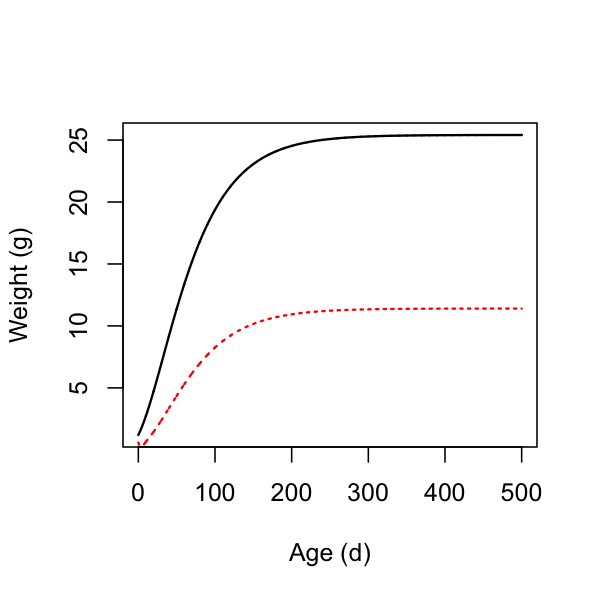
\includegraphics[width=\linewidth]{figure/unnamed-chunk-2-1} \hfill{}

\caption[Proving that this parameter set produces something vaguely mouselike]{Proving that this parameter set produces something vaguely mouselike. This set of parameters yields a healthy mouse that eats 7 g of food per day, has 25g of structural biomass and 7 g of reserve biomass, and at any point will have about 4g of food in its guts.\label{fig:unnamed-chunk-2}}
\end{figure}


\end{knitrout}

\begin{knitrout}\scriptsize
\definecolor{shadecolor}{rgb}{0.969, 0.969, 0.969}\color{fgcolor}\begin{figure}

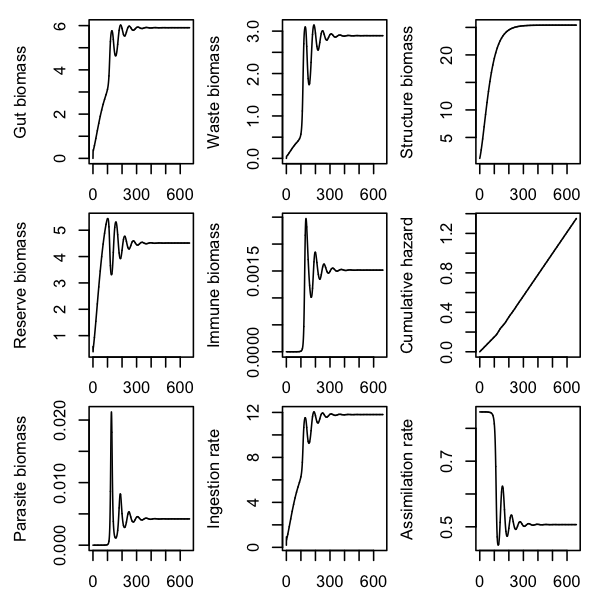
\includegraphics[width=\linewidth]{figure/unnamed-chunk-3-1} \hfill{}

\caption[Results of a model with both consitutive and induced immune response]{Results of a model with both consitutive and induced immune response.\label{fig:unnamed-chunk-3}}
\end{figure}


\end{knitrout}

\bibliographystyle{ecology.bst}
\bibliography{Biblio.bib}

\end{document}
